\documentclass[notitlepage,a4paper,10pt]{article}

% \usepackage{mathpazo} 
\usepackage{ngerman} 
\usepackage[latin1]{inputenc} 
\usepackage[T1]{fontenc} 
\usepackage[pdftex]{graphicx} 
\usepackage[pdftex,bookmarks=true,colorlinks,linkcolor=blue,urlcolor=blue,citecolor=blue]{hyperref}

\sloppy

%opening
\title{I2P - Invisible Internet Project}
\author{Karsten N.}
\date{\today}

\hypersetup {
    pdftitle= { I2P - Invisible Internet Project }
    pdfkeywords= {I2P eepsite SusiMail Bote I2Psnark }
}


\begin{document}
\maketitle
\begin{abstract}
Das Invisible Internet Project (I2P) hat das Ziel, Anonymit�t sowohl f�r Konsumenten als auch f�r Anbieter von Angeboten zu bieten. Dieses Ziel l�sst sich nur in einem geschlossenen Netz verwirklichen.\\

Das Projekt bietet einen Java-basierten Client. Dieser Client verschl�sselt den gesamten Datenverkehr. Au�erdem stellt er sicher, dass st�ndig neue Verbindungen zu anderen Rechnern des Netzwerkes aufgebaut werden.\\

Neben der M�glichkeit, anonym zu surfen und Websites (sogenannte \textit{eepsites}) anzubieten, sind weitere Anwendungen bereits fester Bestandteil von I2P. Es bietet anonyme E-Mail (Susimail, I2P-Bote), BitTorrent Downloads (I2Psnark), ein anonymes Usenet (Syndie) u.a.m.

\end{abstract}
\newpage
\section{Invisible Internet Project}


\subsection{Installation des I2P-Routers}
F�r die Nutzung des Invisible Internet Projects ben�tigt man den I2P-Router, der als Proxy f�r verschiedene Anwendungen (Webbrowser, E-Mail Client...) dient und die Weiterleitung der Daten vom und zum I2P-Netz �bernimmt. Der I2P-Router ist eine Java-Applikation und steht unter \href{http://www.i2p2.de}{www.i2p2.de} zum Download bereit.\\

\begin{description}
 \item[Windows:] Als erstes ist ein Java-Runtime-Environment (JRE) zu installieren. Das Installationsprogramm f�r Java gibt auf der Webseite www.java.com\footnote{ \href{http://www.java.com/de/}{http://www.java.com/de/}}. Der Installer m�chte unbedingt die \textit{Ask-Toolbar} f�r alle Browser installieren. Das sollte man deaktivieren, braucht man nicht.\\

 WICHTIG: Der Installer aktiviert auch ein Java-Plugin f�r alle Browser. Dieses Plug-in ist ein Sicherheitsrisiko und muss im Java Control Panel unter \textit{Systemsteuerung - Programme - Java} deaktiviert werden!
\begin{center}
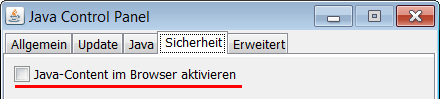
\includegraphics[scale=0.55]{../screenshots/java-ctrl-klein.png}
\end{center}

 Anschlie�end kann der I2P-Router installiert werden. Die Datei \textit{i2pinstall-0.x.y.exe} von der I2P Downloadseite \href{http://www.i2p2.de/download.html}{http://www.i2p2.de/download.html} enth�lt einen kompletten Installer, der nach dem Start alles N�tige einrichtet. Einfach starten und dem Assistenten folgen. Nach der Installation findet man im Startmen� die neue Gruppe \textit{I2P} (Bild \ref{abb:i2pstartwin}).\\
 
  \begin{figure}[htb]
  \begin{center}
  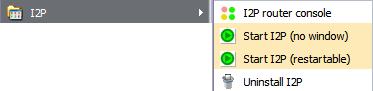
\includegraphics[scale=0.60]{../screenshots/i2p-win.png}
  \caption{I2P im Startmen� von Windows}
  \label{abb:i2pstartwin}
  \end{center}
  \end{figure}

Die beiden Punkte zum Starten von I2P unterscheiden sich nur gering. Im ersten Fall hat man keine st�rende Konsole auf dem Desktop. \textit{I2P router console} �ffnet den Webbrowser, um den Router zu konfigurieren oder abzuschalten mit der Adresse \href{http://localhost:7657}{http://localhost:7657}.

\item[Ubuntu:] F�r Ubuntu kann man das offizielle PPA Repository der I2P Maintainer nutzen. Dieses Repository enth�lt nur den I2P-Router. Es wird mit folgenden Kommandos aktiviert und danach der I2P-Router installiert: 
\begin{verbatim}
  > sudo apt-add-repository ppa:i2p-maintainers/i2p
  > sudo apt-get update
  > sudo aptitude install i2p 
\end{verbatim}
Au�erdem gibt es das I2P PPA-Repository von KYTV. Dieses Repository enth�lt neben dem I2P-Router weitere n�tzliche Software wie I2P-Bote. Das Repository wird mit folgendem Kommando aktiviert: 
\begin{verbatim}
  > sudo apt-add-repository ppa:i2p.packages/i2p
\end{verbatim}
Danach kann man wie �blich alles n�tige auf die Platte sp�len: 
\begin{verbatim}
  > sudo apt-get update
  > sudo aptitude install i2p i2p-bote
\end{verbatim}

\item[Linux:]  Installieren Sie als erstes Java (Paket: \textit{default-jre}) mit der Paketverwaltung der Distribution. Anschlie�end kann der I2P-Router installiert werden. Den Installer \textit{i2pinstall-0.x.y.jar} findet man auf der Downloadseite des Projektes\footnote{ \href{http://www.i2p2.de/download.html}{http://www.i2p2.de/download.html}}. Nach dem Downlad startet man den Installer und w�hlt die Sprache sowie Verzeichnis f�r die Installation:
\begin{verbatim}
 > java -jar i2pinstall-*.jar
\end{verbatim}
In dem neu angelegten Installationsverzeichnis findet man das Script zum Starten/Stoppen des I2P-Routers:
\begin{verbatim}
 > ~/i2p/i2prouter start
\end{verbatim}

Stoppen l�sst sich der Router in der Router-Konsole im Webbrowser unter  \href{http://localhost:7657}{http://localhost:7657} mit Klick auf den Link \textit{shutdown} oder obiges Kommando mit der Option \textit{stop}.

\item[Linux (advanced):] K. Raven hat eine umfassende Anleitung geschrieben, wie man den I2P-Router in einer chroot-Umgebung installiert und mit AppAmor zus�tzlich absichert. Lesenswert f�r alle, die es richtig gut machen wollen. Link: \href{http://wiki.kairaven.de/open/anon/chrooti2p}{http://wiki.kairaven.de/open/anon/chrooti2p}
\end{description}

Nach dem ersten Start braucht der I2P-Router einige Zeit, im sich im Invisible Internet zu orientieren. Zum Warmlaufen sollte man ihm 30min Zeit lassen. Wenn es danach noch immer nicht so richtig funktioniert, sind die Netzwerkeinstellungen zu pr�fen. Die Startseite der Router-Console gibt einige Hinweise.\\

Den I2P-Router kann man nicht kurz einmal starten, wenn man ihn nutzen m�chte. Er sollte m�glichst immer laufen, wenn der Rechner online ist. Damit lernt er die verf�gbaren Peers und eepsites besser kennen und ist besser in das Netz eingebunden.

\subsection{Konfiguration des I2P-Router}
Standardm��ig ist der I2P-Router funktionsf�hig vorkonfiguriert. Ein paar kleine Anpassungen k�nnen die Arbeit etwas verbessern.

\subsubsection*{Bandbreite anpassen}
Der I2P-Router arbeitet am besten, wenn man die Bandbreite an den eigenen Internetanschluss anpasst. Nach dem Start kann man auf der Seite \href{http://localhost:7657/config}{http://localhost:7657/config} der Router Konsole die Werte anpassen. 

\subsubsection*{Netzwerk Konfiguration}
Auf der Seite \href{http://localhost:7657/confignet}{http://localhost:7657/confignet} der Router Konsole sind die Einstellungen f�r die Einbindung in das I2P-Netz zu konfigurieren. Dabei gibt es zwei M�glichkeiten: 
\begin{enumerate}
 \item Wenn der eigene Rechner nicht vom Internet erreichbar ist, dann sind folgende Optionen zu aktivieren, damit der I2P-Router korrekt arbeitet: 
  \begin{itemize}
   \item \textit{Versteckter Modus} ist zu aktivieren.
   \item Optional kann der \textit{Laptop Modus} aktiviert werden. Dann �ndert sich Router-Identifikation bei �nderung der IP-Adresse.
  \end{itemize}
 \item Wenn der eigene I2P-Router vom Internet f�r andere Teilnehmer erreichbar ist, verbessert sich die Performance und Anonymit�t. In der Netzwerk Konfiguration des I2P-Routers sind dann folgende Optionen zu konfigurieren: 
  \begin{itemize}
   \item UPnP ist aus Sicherheitsgr�nden auf dem DSL-Router zu deaktivieren. Damit ist klar, dass in der Netzwerk Konfiguration des I2P-Routers das \textit{UPnP Portforwarding} und die \textit{UPnP IP-Adresserkennung} auch zu deaktivieren sind.
   \item In den UDP-Einstellungen ist der Port anzugeben, f�r den die Weiterleitung auf dem DSL-Router konfiguriert wurde.
   \item n den TCP-Einstellungen ist ebenfalls der Port zu konfigurieren und die Option \textit{automatisch erkannte IP-Adresse benutzen} zu aktivieren.
  \end{itemize}
Die Hinweise im Kapitel \textit{Konfiguration des DSL-Routers} erl�utern die notwendigen Einstellungen, damit Ihr Rechner vom Internet erreichbar ist. Auf dem DSL-Router ist ein Portforwarding zu Ihrem Rechner zu konfigurieren und die Firewall des Rechners ist anzupassen. 
\end{enumerate}


\subsubsection*{SusiDNS anpassen}
F�r die Zuordnung von Domain Namen mit der Toplevel Domain .i2p zu einem Service wird SusiDNS verwendet, ein dem DNS im Internet vergleichbares System. Wie in den Anfangszeiten des WWW erh�lt jeder I2P Router eine komplette Liste der bekannten eepsites, das \textit{addressbook}.\\

Um neue eepsites oder Services in das addressbook einzuf�gen, verwendet I2P sogenannte \textit{subscriptions}. Die eine standardm��ig vorhandene subscription wird relativ selten aktualisiert.\\

Um auf dem Laufenden zu bleiben, kann man weitere subscriptions zu abonnieren. Die Einstellungen f�r SusiDNS findet man in der Router Konsole. Subscriptions kann man unter folgender Adresse einf�gen: \href{http://localhost:7657/susidns/subscriptions.jsp}{http://localhost:7657/susidns/subscriptions.jsp} (Bild \ref{susidns})\\

\begin{figure}[htb]
\begin{center}
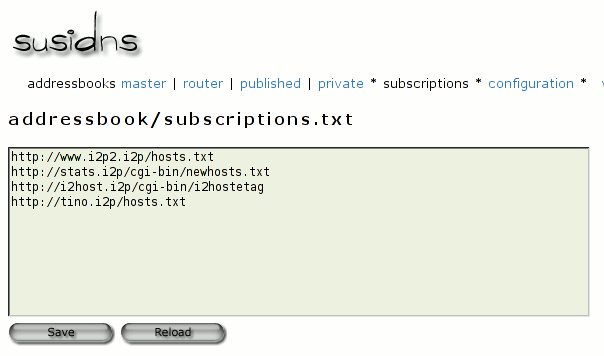
\includegraphics[scale=0.50]{../screenshots/susidns.png}
\caption{subscriptions f�r SusiDNS}
\label{susidns}
\end{center}
\end{figure}

Folgende subscriptions bieten aktuelle Neuerscheinungen von eepsites:
\begin{verbatim}
 http://stats.i2p/cgi-bin/newhosts.txt
 http://i2host.i2p/cgi-bin/i2hostetag
 http://tino.i2p/hosts.txt
\end{verbatim} 

\subsection{Anonym Surfen mit I2P}
Der I2P-Router stellt einen HTTP- und HTTPS-Proxy f�r den Webbrowser bereit.
 Die Default-Adressen dieser Proxys sind:
\begin{verbatim}
             Rechner:  localhost
     HTTP-Proxy Port:  4444
      SSL-Proxy Port:  4445
      FTP-Proxy Port:  4444
   Gopher-Proxy Port:  4444
\end{verbatim}

Der Proxy kann genutzt werden, um Webseiten im Invisible Internet aufzurufen (sogenannte \textit{eepsites}, erkennbar an der Toplevel Domain \textbf{.i2p}).

\subsubsection*{JonDoFox nutzen}

Das Firefox Profil \textit{JonDoFox} ist f�r spurenarmes uns sicheres Surfen optimiert. Es bietet neben \textit{JonDo} und \textit{Tor} eine \textit{Benutzerdefinierte Proxy Konfiguration}, die man f�r I2P nutzen kann. Die Einstellungen  zeigt Bild \ref{i2pjondofox}. Der JonDoFox verhindert zuverl�ssig eine Kompromittierung der Anonymit�t. 

\begin{figure}[htb]
\begin{center}
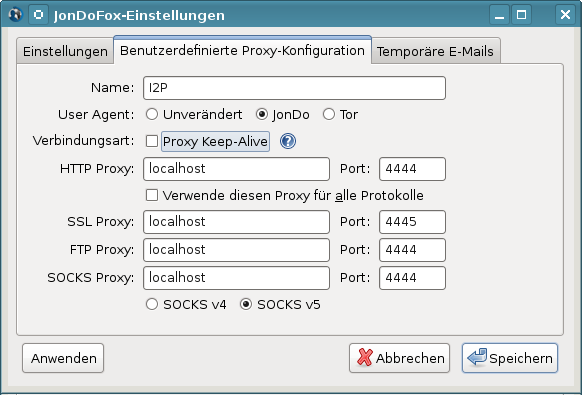
\includegraphics[scale=0.75]{../screenshots/i2p-jondofox.png}
\caption{Benutzerdefinierte Proxy Konfiguration im JonDoFox}
\label{i2pjondofox}
\end{center}
\end{figure}

\subsubsection*{Firefox selbst konfigurieren}
Ich w�rde empfehlen, f�r das Surfen im Invisible Internet ein separates Firefox-Profil zu erstellen. Dann ist es f�r spionierende Websites g�nzlich unm�glich, im Cache oder in der Historie abgelegte Daten �ber das anonyme Surfen auszulesen. Den Profil-Manager von Firefox startet man mit folgendem Kommando:
\begin{verbatim}
 > firefox -P
\end{verbatim} 
In dem sich �ffnenden Dialog (Bild \ref{i2pffstart}) kann man ein neues Profil anlegen und anschlie�end die Proxy-Einstellungen konfigurieren. In Zukunft wird Firefox bei jedem Start fragen, welches Profil genutzt werden soll.\\

\begin{figure}[htb]
\begin{center}
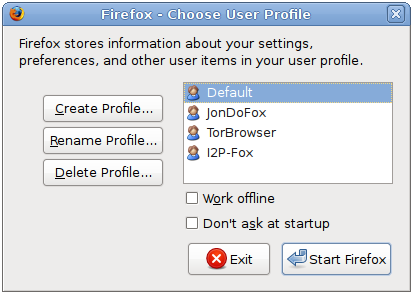
\includegraphics[scale=0.55]{../screenshots/vmware-ff-start.png}
\caption{Firefox Profil-Manager}
\label{i2pffstart}
\end{center}
\end{figure}

Anschlie�end kann das Profil \textit{I2P-Fox} gestartet werden und die Proxy-Einstellungen sind wie im Bild \ref{i2pffprivat} gezeigt zu konfigurieren. Die allgemeinen Hinweise zu Cookies, Javascript, Plug-Ins, HTTPS-Security usw. im Abschnitt \textit{Spurenarm Surfen} gelten auch f�r I2P. Das Profil \textit{I2P-Fox} ist entsprechend zu konfigurieren.\\

\begin{figure}[htb]
\begin{center}
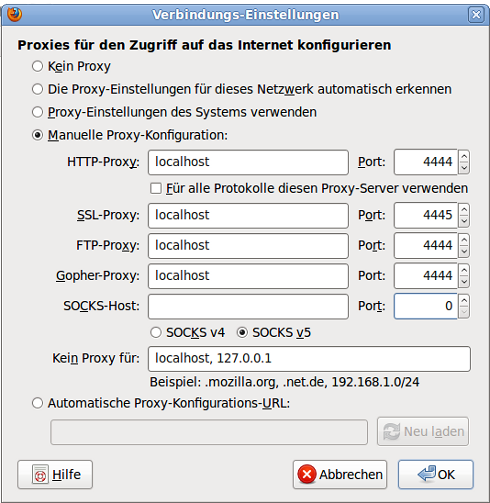
\includegraphics[scale=0.7]{../screenshots/i2p-proxy-einstellungen.png}
\caption{Firefox Proxy-Einstellungen f�r I2P}
\label{i2pffprivat}
\end{center}
\end{figure}

\subsubsection*{Wichtige Sicherheitseinstellungen f�r Firefox}
Flash und Java Plug-ins sind unbedingt zu deaktivieren, da diese Plug-ins die Proxy Einstellungen umgehen k�nnten. Um eine Deanonymisierung zu vermeiden, sind f�r einen aktuellen Firefox au�erdem folgende Features unter der Adresse \textit{about:config} zu deativieren:
\begin{itemize}
 \item Websockets leaken DNS-Requests:
\begin{verbatim}
    network.websocket.enabled = false
\end{verbatim} 
 \item WebRTC kann durch UDP-Tunnel die reale IP-Adresse aufdecken (nur Firefox 18 und neuer):
\begin{verbatim}
    media.peerconnection.enabled = false
\end{verbatim} 
\item Geolocation-API kann den realen Standort ermitteln:
\begin{verbatim}
    geo.enabled = false
\end{verbatim} 
\item Phishing- und Malware Protection funktioniert f�r eepsites nicht, da die Webseiten des Darknet nicht in der Google Datenbank enthalten sind:
\begin{verbatim}
    browser.safebrowsing.enabled = false
\end{verbatim} 
\end{itemize}


\subsubsection*{Suchmaschinen f�r I2P}
Um sich in einem Netzwerk zu orientieren, braucht man eine Suchmaschine. Die Webseite plugins.i2p bietet viele \textit{Firefox Search Plugins f�r I2P}. Wenn man die Webseite \href{http://plugins.i2p/firefox/}{http://plugins.i2p/firefox} aufgerufen hat, kann man die Suchmaschinen einfach durch Aufklappen der Liste der Suchmaschinen oben rechts im Firefox hinzuf�gen. Unter dem Trennstrich findet man die neuen Suchmaschinen, die diese Webseite zur Installation anbietet.\\

Das �quivalent zu Google im normalen Internet ist im I2P-Netz die Suchmaschine \href{http://eepsites.i2p/}{http://eepsites.i2p}. Die anderen Dienste in der Liste durchsuchen einzelne eepsites. 

\subsection{I2P Mail 1 (Susimail)}
Die Anwendung Susimail ist integraler Bestandteil von I2P und erm�glicht den unbeobachteten Austausch von E-Mails. Das Anlegen und Verwalten eines Susimail-Accounts erfolgt auf der eepsite \href{http://hq.postman.i2p}{http://hq.postman.i2p}.\\

Es ist m�glich, E-Mails in das normale Web zu versenden und auch von dort unter der Adresse \textit{<username>@i2pmail.org} zu empfangen. In Abh�ngigkeit der auf HQ Postmaster gew�hlten Einstellungen kann dieser �bergang ins normale Internet bis zu 24h dauern. Um f�r Spammer unattraktiv zu sein, haben die Entwickler von I2P die Anzahl der ins normale Web versendbaren Mails begrenzt. Es ist m�glich, innerhalb von 24h bis zu 20 Emf�ngern beliebig viele E-Mail zu senden. Wer unbedingt mehr Leute per E-Mail kontaktieren will, kann mit einem Hashcash ein Kontingent von weiteren 20, 40 oder 80 Empf�ngern freischalten.

\subsubsection*{Router-Konsole nutzen}
Ein einfaches Webinterface f�r Susimail ist in der I2P Router Konsole erreichbar unter der Adresse \href{http://localhost:7657/susimail/susimail}{http://localhost:7657/susimail/susimail}.\\

\begin{figure}[htb]
\begin{center}
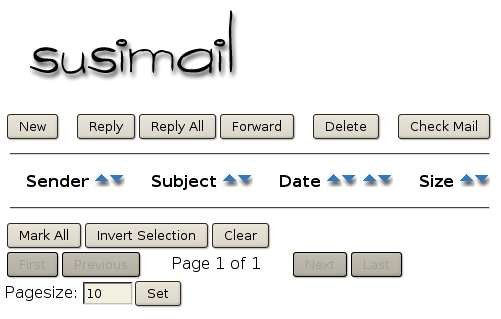
\includegraphics[scale=0.70]{../screenshots/susimail.png}
\caption{Webinterface von Susimail}
\end{center}
\end{figure}

Es bietet eine simple M�glichkeit, Mails abzurufen und zu versenden. Komfortabler ist die Nutzung des bevorzugten E-Mail Clients, vor allem wenn man die M�glichkeiten zur Verschl�sselung der Nachrichten nutzen m�chte.

\subsubsection*{Thunderbird konfigurieren}
Der Susimail-Account kann mit jedem E-Mail Client genutzt werden.

\begin{verbatim}
    SMTP-Server: localhost    Port: 7659
    POP3-Server: localhost    Port: 7660
    Login-Name:  <username>
\end{verbatim} 

In Thunderbird ist als erstes ein neuer SMTP-Server anzulegen (Konten -> Postausgangs-Server (SMTP) -> Hinzuf�gen). Der Server erfordert eine Authentifizierung mit dem Daten des Susimail Accounts.\\

Danach kann ein neues POP3-Konto angelegt werden, welches diesen SMTP-Server f�r die Versendung nutzt. SSL- und TLS-Verschl�sselung sind zu deaktivieren. Der I2P-Router �bernimmt die abh�rsichere �bertragung.\\

In den Server-Einstellungen des Kontos sollte die Option \textit{``Alle x Minuten auf neue Nachrichten pr�fen''} deaktiviert werden! Die Admins von Susimail bitten darum, den Service nicht unn�tig zu belasten.

\subsubsection*{Susimail mit Tor nutzen}
An Stelle des I2P-Routers kann auch Tor f�r den Abruf und das Versenden von Nachrichten via I2P Mail genutzt werden. Folgende Hidden Services bieten ein SMTP-Gateway (Port: 7659) und POP3-Gateway (Port: 7660):

\begin{verbatim}
    v6ni63jd2tt2keb5.onion
    5rw56roal3f2riwj.onion
\end{verbatim}

Die Hidden Service Adresse ist als SMTP- und POP3-Server im E-Mail Client f�r das I2P-Mail-Konto an Stelle von \textit{localhost} einzutragen. Au�erdem ist der E-Mail Client so zu konfigurieren, dass er Tor als Proxy nutzt. Sollte der E-Mail Client st�ndig den Fehler TIMEOUT liefern, hilft es, den Hidden Service erst einmal im Webbrowser aufzurufen.

\subsubsection*{Hinweise zur Nutzung von Susimail}
Der Service wird von \textit{postman} und \textit{mastijaner} in der Freizeit aufgebaut und gepflegt. Sie bitten darum, folgene Hinweise zu beachten:
\begin{enumerate}
 \item Bitte nicht den POP3-Service in kurzen Intervallen automatisiert abfragen. Einige Nutzer fragen den POP3-Dienst immer wieder innerhalb weniger Minuten ab und belasten den Service stark. Zweimal pro Tag sollte reichen.
\item Um anonym zu bleiben, sollte man keine Mails an die eigene Mail Adresse im Web schreiben oder an Bekannte, mit denen man via E-Mail im normalen Web Kontakt h�lt.
\item Bitte Susimail nicht f�r Mailinglisten nutzen, die man nicht mitliest. Das Abmelden auf Mailinglisten bei Desinteresse nicht vergessen.
\item Wer nicht mehr im Invisible Internet aktiv ist, sollte auch an das L�schen des Susimail Account denken. Scheinbar gibt es auf dem Server viele tote Mail-Accounts, wo noch immer Mails eingehen (Spam und Mailinglisten) und viel Speicherplatz verbrauchen.
\item Bitte verwendet den Dienst nicht, um anonyme Beleidigungen oder Drohungen zu schreiben. Das bringt den Betreibern �rger und gef�hrdet den reibungslosen Betrieb.
\end{enumerate}
Englischer Orginaltext bei HQ Postman: \href{http://hq.postman.i2p/?p=63}{http://hq.postman.i2p/?p=63}

\subsection{I2P Mail 2 (Bote)}
I2P Bote bietet serverlose und verschl�sselte E-Mail Kommunikation. Die Daten werden redundant und verschl�sselt in einer DHT gespeichert, �ber alle Teilnehmer verteilt. Es gibt keinen zentralen Server, der Kommunikationsprofile erstellen oder eine Vorrats�daten�speicherung umsetzen k�nnte. Starke Kryptografie stellt sicher, dass nur der Empf�nger die Nachricht lesen kann.\\

I2P Bote ist keine Weiterentwicklung von Susimail und es soll es auch nicht ersetzen. Langfristig werden beide Projekte parallel existieren und kooperieren. Das Projekt bietet folgende Features:
\begin{itemize}
\item Bedienung im Webinterface der I2P-Router Konsole.
\item Erzeugen von Identit�ten, Senden/Empfangen von E-Mails.
\item Anonyme Absender und Versenden �ber Zwischenstationen mit zeitlicher Verz�gerung (Remailer-Konzept).
\item Dateianh�nge bis 500 kB werden unterst�tzt. Die Begrenzung der Gr��e der Dateianh�nge ist aufgrund der redundanten Speicherung n�tig. Die Nachrichten werden mit 20x Redundanz gespeichert und eine 1 MB gro�e Mail w�rde 20 MB Speicherplatz in der DHT belegen.
\end{itemize}

\subsubsection*{Installation von I2P Bote}
Um I2P Bote zu nutzen, ist die Installation von 3 Plug-Ins f�r den I2P Router n�tig. Auf der Seite I2P Dienste der Router Konsole (unter \href{http://localhost:7657/configclients.jsp}{http://localhost:7657/configclients.jsp}) findet man ganz unten den Abschnitt f�r die Installation zus�tzlicher Plug-Ins (Bild \ref{i2pbote1}).\\

\begin{figure}[htb]
\begin{center}
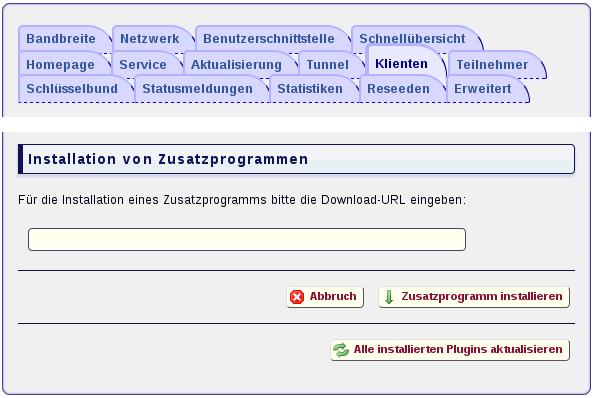
\includegraphics[scale=0.70]{../screenshots/i2pbote_1.png}
\caption{Installation des Plug-in I2P Bote}
\label{i2pbote1}
\end{center}
\end{figure}

Folgende Plug-Ins sind in dieser Reihenfolge zu installieren: 
\begin{enumerate}
 \item \href{http://sponge.i2p/files/seedless/01\_neodatis.xpi2p}{http://sponge.i2p/files/seedless/01\_neodatis.xpi2p}
 \item \href{http://sponge.i2p/files/seedless/02\_seedless.xpi2p}{http://sponge.i2p/files/seedless/02\_seedless.xpi2p}
 \item \href{http://i2pbote.i2p/i2pbote.xpi2p}{http://i2pbote.i2p/i2pbote.xpi2p}
\end{enumerate}

Nach erfolgreicher Installation findet man auf der Startseite in der Liste der \textit{Lokalen Dienste} oder rechts im Men� der Routerkonsole einen neuen I2P Dienst \textit{SecureMail}. Ein Klick �ffnet die Web-Oberfl�che in einem neuen Browser-Tab. 

\subsubsection*{Eigene Identit�t erzeugen}
Der erste Schritt nach der Installation ist in der Regel die Erstellung einer eigenen Adresse. In der Navigationsleiste rechts w�hlt man \textit{''Identit�ten''} und den Button \textit{``Neue Identit�t''}.\\

Als Pflichtfeld ist nur ein Name anzugeben. Die Verschl�sselung bel�sst man am besten bei 256Bit-ECC. Diese Verschl�sselung liefert relativ kurze und starke Schl�ssel. Die Mail�adresse wird zur Zeit noch nicht genutzt.\\

Die kryptische Bote-Adresse ist an alle Partner zu verteilen oder zu ver�ffentlichen. In der �bersicht ist die Adresse nicht voll sichtbar. Wenn man auf die Identit�t klickt, erh�lt man eine vollst�ndige Ansicht. Die gesammelten Adressen der Partner k�nnen in einem rudiment�ren Adressbuch verwaltet werden. 

\begin{figure}[htb]
\begin{center}
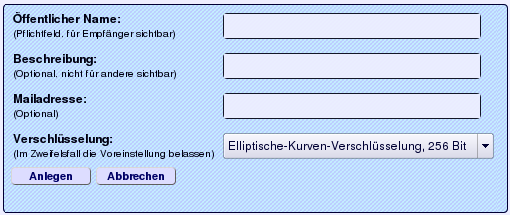
\includegraphics[scale=0.70]{../screenshots/i2pbote_3.png}
\caption{Neue Ident�t f�r I2P-Bote anlegen}
\label{i2pbote3}
\end{center}
\end{figure}

\subsubsection*{Konfiguration}
Bevor man loslegt, sollte man einen Blick in die Konfiguration werfen und diese anpassen. 
\begin{itemize}
 \item Abrufen der Nachrichten: Es ist konfigurierbar, ob und in welchem Intervall neue Nachrichten aus der DHT automatisch abgerufen werden sollen. Um die Belastung des Bote-Netzes gering zu halten sollte man Intervalle von 2-3h nutzen. Bei Bedarf kann man das Abrufen neuer Nachrichten auch selbst ansto�en.

 \item �ber Zwischenstationen senden: Wird diese Option deaktiviert (``AUS``), gehen versendete Nachrichten direkt in die DHT. Die Anonymit�t entspricht der normalen Anonymit�t bei der Nutzung von I2P.\\

Eine h�here Anonymit�t erreicht man, wenn die Nachricht vor dem Speichern in der DHT �ber 1\dots n Teilnehmer des I2P-Bote Netzes geleitet und dort jeweils um eine zuf�llige Zeitspanne verz�gert wird. Die min. und max. Werte f�r die Verz�gerung k�nnen konfiguriert werden. �hnlich wie bei Remailern sinkt damit nat�rlich die Performance der Kommunikation. 

 \item Durchleitung an Nicht-I2P-Adressen: Es ist m�glich, Mails an Nicht-I2P-Bote Teilnehmer zu versenden. Die Nachrichten werden an die Bote-Adresse eines Durchleitungsdienstes versendet, der sich dann um die weitere Zustellung k�mmert. Derzeit arbeitet HQ Postman an der Entwicklung dieses Services, der aber noch nicht arbeitsf�hig ist.

 \item Absendezeit: Die Absendezeit sollte man nicht mit versenden, wenn die Nachricht �ber Zwischenstationen gesendet wird. Anderenfalls ist es ein Feature, dass die Anonymit�t nur geringf�gig erh�hen kann, wenn diese Option deaktiviert wird. Mir hilft es, den �berblick in der Inbox zu behalten, wenn ein Zeitstempel vorhanden ist.
\end{itemize}

\subsubsection*{Mails schreiben und empfangen}
Das im Bild \ref{i2pbote2} gezeigte Formular f�r eine neue Mail �ffnet sich mit Klick auf den Button \textit{``Neu''}.\\

\begin{figure}[htb]
\begin{center}
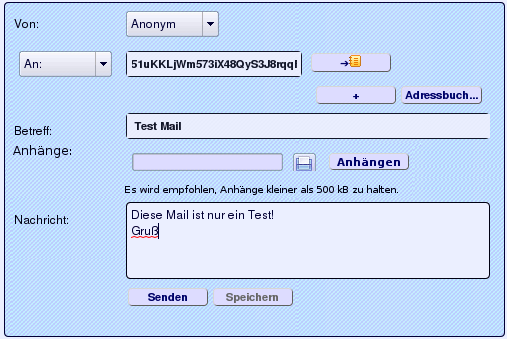
\includegraphics[scale=0.70]{../screenshots/i2pbote_4.png}
\caption{Neue E-Mail in I2P Bote schreiben}
\label{i2pbote2}
\end{center}
\end{figure}

Als Absender kann man \textit{Anonym} w�hlen, oder eine der zuvor angelegten Identit�ten. Wer \textit{Anonym} w�hlt, sollte sich nicht wundern, dass er vom Empf�nger als anonymer Unbekannter behandelt wird. F�r vertrauliche Konversation muss man seinen Gegen�ber verifizieren k�nnen.\\

In die Felder \textit{An}, \textit{Kopie} oder \textit{Blindkopie} sind die kryptischen Bote-Adressen der Empf�nger einzutragen, der Rest sollte sich selbst erkl�ren.\\

Eingehende Mails findet man im Ordner \textit{Posteingang} und weitere Fragen beantworten bestimmt die FAQ von I2P Bote \footnote{ \href{http://i2pbote.net/faq.html}{http://i2pbote.net/faq.html}}.

\subsubsection*{Adressbuch}
Das Web-Interface bietet ein einfaches Adressbuch. Man kann die Bote-Adressen und Namen von Partnern sammeln und beim Schreiben einer Mail mit zwei Klicks �bernehmen.\\

Au�erdem hilft das Adressbuch bei der Verifikation der Absender empfangener Nachrichten. Ein Absender ist eindeutig nur durch seine Bote-Adresse bestimmt. Der Name kann frei gew�hlt werden und kann auch mehrfach genutzt werden. Es k�nnte also jemand den Namen HungryHobo nutzen, um sich als Hauptentwickler von I2P-Bote auszugeben.\\

Ein Vergleich der Bote-Adressen ist nicht intuitiv. Das Adressbuch kann diese Aufgabe �bernehmen. Ist der Absender einer Nachricht im Adressbuch enthalten und stimmt die Bote-Adresse �berein, dann zeigt die Liste der Inbox ein H�ckchen in der Spalte \textbf{Bek}.

\begin{figure}[htb]
\begin{center}
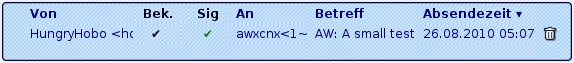
\includegraphics[scale=0.70]{../screenshots/i2pbote_6.png}
\caption{Inbox mit verifiziertem Absender}
\label{i2pbote6}
\end{center}
\end{figure}


\subsection{I2P IRC}
IRC ist ein �ffentlicher Chat Service. Auf den IRC-Servern gibt es verschiedene Chat-R�ume, sogenannte Channels, in denen man sich zu einem bestimmten Thema austauschen kann. Die Unterhaltung ist in der Regel �ffentlich, aber auch private Nachrichten k�nnen zwischen Nutzern ausgetauscht werden.\\

Das I2P-Netz bietet zwei anonyme Chat-Server, die direkt �ber den I2P-Router erreichbar sind. Die Konfiguration der verschiedenen Clients wie XChat (Linux/UNIX), Kopete (KDE), Colloquy (MacOS) oder Mirc (Windows) ist einfach. Man nutzt als Chat-Server folgende Adresse und ist anonym:  
\begin{verbatim}
 Host: localhost
 Port: 6668
\end{verbatim}

\subsubsection*{Die wichtigsten Chat-Kommandos}
Der Chat wird in der Regeln komplett durch Kommandos gesteuert. Alle Kommandos beginnen mit einem Slash. Eine kurze Liste der wichtigen Kommandos:
\begin{description}
 \item[/list] Listet alle Diskussions-Channels auf, die auf dem Server verf�gbar sind.
 \item[/join \#channel] Den Raum \#channel betreten und mitdiskutieren.
 \item[/quit] Den aktiven Raum verlassen oder vom Server abmelden.
 \item[/msg nick <text>] Sendet eine Nachricht an den User \textit{nick}.
 \item[/ignore nick] Einen Troll ignorieren.
 \item[/help] Beantwortet alle weiteren Fragen.
 \end{description}
Im IRC ist man man einem Nicknamen unterwegs. Die Nicknamen werden registriert und mit einem Passwort gesch�tzt, damit kein Dritter einen bekannten Nicknamen nutzen kann, um sich eine Identit�t zu erschleichen.\\

Die Registrierung erfolgt mit folgendem Kommando:
\begin{verbatim}
  /msg nickserv register <Password> fake-email-addr
\end{verbatim}
Um einen registrierten Nicknamen zu nutzen, muss man sich identifizieren: 
\begin{verbatim}
  /msg nickserv identify <Password>
\end{verbatim}

\subsubsection*{\#anonops}
Die Channels von \textit{Anonymous} stehen auch auf den I2P-IRC Servern zur Verf�gung. F�r die Diskussionen in diesen Channels sollten sie die Regeln von \textit{Anonymous} beherzigen:\\

\textit{Basics: Tauchen Sie in der Masse unter ohne ein besonders smarter Typ sein zu wollen. Es gibt keine Helden, die alt geworden sind, es gibt nur junge Helden und ``tote`` Helden.}\\
 
Geben sie keine pers�nlichen Informationen im public IRC preis.
\begin{itemize}
 \item keine Anhaltspunkte im Nicknamen und Realnamen ver�ffentlichen
 \item keine pers�nlichen Informationen im Chat diskutieren
 \item keine Informationen �ber die Herkunft diskutieren (Land, Stadt usw.)
 \item keine Beschreibung von Tattoos, Piercings oder anderer Merkmale
 \item keine Informationen �ber Beruf und Hobbys
 \item keine Sonderzeichen wie ��� verwenden, die nur in Ihrer Sprache verf�gbar sind
 \item ver�ffentlichen Sie nichts im normalen Netzm w�hrend Sie in einem anonymen Chat sind, es kann einfach korreliert werden
 \item posten Sie keine Bilder von Facebook im Chat, diese Bilder enthalten die pers�nliche ID
 \item verbinden Sie sich nicht Tag f�r Tag zur gleichen Zeit mit dem Chat
\end{itemize}

\subsection{I2P BitTorrent}
Der I2P-Router bietet auch eine angepasste Implementierung des BitTorent Protokolls f�r anonymes Peer-2-Peer Filesharing. Im Gegensatz zur Nutzung von normalem BitTorrent �ber Tor ist die Implementierung des Invisble Internet Project anonym und die Nutzung ausdr�cklich erw�nscht. Der Dienst bietet Optimierungen mit speziellen Clients.\\

Die I2P-Router-Konsole bietet einen einfachen BitTorrent Client als Webinterface unter \textit{Torrents} (\href{http://localhost:7657/i2psnark}{http://localhost:7657/i2psnark}).\\

Die zum Tausch bereitgestellten oder heruntergeladenen Dateien findet man im Unterverzeichnis \textit{i2psnark} der I2P-Installation. Dieses Verzeichnis sollte Lese- und Schreibrechte f�r alle lokalen User haben, die I2PSnark nutzen d�rfen. Torrents findet man z.B. auf den eepsites \href{http://tracker2.postman.i2p}{http://tracker2.postman.i2p}, \href{http://crstrack.i2p/tracker}{http://crstrack.i2p/tracker} oder \href{http://tracker.welterde.i2p}{http://tracker.welterde.i2p}. Das Webinterface bietet direkte Links zu diesen eepsites.\\

\textbf{Hinweis zur Nutzung:} Es geh�rt beim Filesharing zum guten Ton, Dateien nicht nur zu saugen. Man stellt die heruntergeladenen Dateien auch anderen Teilnehmern zur Verf�gung. Bei BitTorrent im normalen Netz gilt es als freundlich, wenn man heruntergeladene Dateien mindestens f�r 2 Tage zum Upload anbietet oder bis die Datenmenge des Upload das 2,5fache des Downloads betr�gt. Da die Geschwindigkeit im I2P-Netz wesentlich geringer ist, sollte man herunter geladene Dateien mindestens f�r 1 Woche zum Upload anbieten. 

\end{document}